\documentclass[10pt,titlepage,a5paper]{ltjsbook}
\usepackage{amsmath}
\usepackage{amssymb}
\usepackage{amsfonts}
\usepackage{graphicx}
\usepackage{float}
\usepackage{xcolor}
\usepackage{enumitem}
\usepackage{etoolbox}
\usepackage{subfiles}
\usepackage{cleveref}
\usepackage{tcolorbox}
\usepackage{quotchap}
\usepackage{fancyhdr}
\usepackage{wrapfig}
\usepackage{geometry} % geometry パッケージを読み込む
\geometry{
    a5paper,      % 用紙サイズを再度指定(冗長でも安全のため)
    left=12mm,    % 左の余白を12mmに
    right=12mm,   % 右の余白を12mmに
    top=12mm,     % 上の余白を12mmに
    bottom=12mm,  % 下の余白を12mmに
    %showframe % 余白の境界線を可視化したい場合(最終出力時には削除)
}
\usepackage{titlesec}
\titleformat{\section}[block]{}{}{0pt}
{
  \definecolor{teal}{gray}{0.30}
  \begin{picture}(0,0)
    \put(-10,-5){
      \begin{tikzpicture}
        \fill[teal] (0pt,0pt) rectangle (5pt,19pt);
      \end{tikzpicture}
    }
    \put(-10,-5){
      \color{teal}
      \line(1,0){\hsize}
    }
  \end{picture}
  \hspace{0pt}
  \sffamily \Large \thesection
  \hspace{0pt}
}
\pagestyle{fancy} % fancy スタイルを使用することを宣言

% ヘッダーとフッターのすべてのフィールドをクリア
\fancyhf{}

% 奇数ページ (odd page) のフッター設定
\fancyfoot[LO]{\thepage} % Left Odd: 左下 (ページ番号)
\fancyfoot[RO]{}         % Right Odd: 右下 (空にする)

% 偶数ページ (even page) のフッター設定
\fancyfoot[LE]{}         % Left Even: 左下 (空にする)
\fancyfoot[RE]{\thepage} % Right Even: 右下 (ページ番号)

% ヘッダーとフッターの下線を消す
\renewcommand{\headrulewidth}{0pt} % ヘッダーの下線を0pt (消去)
\renewcommand{\footrulewidth}{0pt} % フッターの上線を0pt (消去)

% chapter の開始ページ(plain スタイル)もフッターにページ番号を表示させる
\fancypagestyle{plain}{
  \fancyhf{} % ヘッダーとフッターをクリア
  \fancyfoot[LO]{\thepage} % 左下 (奇数ページ)
  \fancyfoot[RE]{\thepage} % 右下 (偶数ページ)
  \renewcommand{\headrulewidth}{0pt} % ここにも下線消去を設定
  \renewcommand{\footrulewidth}{0pt} % ここにも下線消去を設定
}
\begin{document}
  %\chapter{屋久島の気候}
  \section{屋久島の降水量}
    屋久島の気候について論ずるとき, その雨量について触れないわけにはいかない. 屋久島は日本で最も雨が降る地域であり, 平地では年間平均雨量が4000mmを超え, 山間部では8000mm-12000mmに達する.
    小説家の林芙美子は屋久島が舞台の小説『浮雲』の中で屋久島は一か月のうち35日雨が降ると書いている. はたから聞くと, 何を言っているんだと思うかもしれない. だが, この表現はなかなかに的を得ていて, 雨の多い時期にはほんとに毎日以上雨が降っているような気さえする. 
    実際, 一日の降水量が400mmを超えることもあり, これは福岡の年平均降水量の約四分の一に相当する. 屋久島に住んでいると, バケツをひっくり返したような雨すらも超えるような, 
    海をひっくり返したような雨を一年に一度は経験することになる. \\
    以下に屋久島とメンバーそれぞれの地元の降水量のグラフを示す.
    \begin{figure}[H]
      \centering
      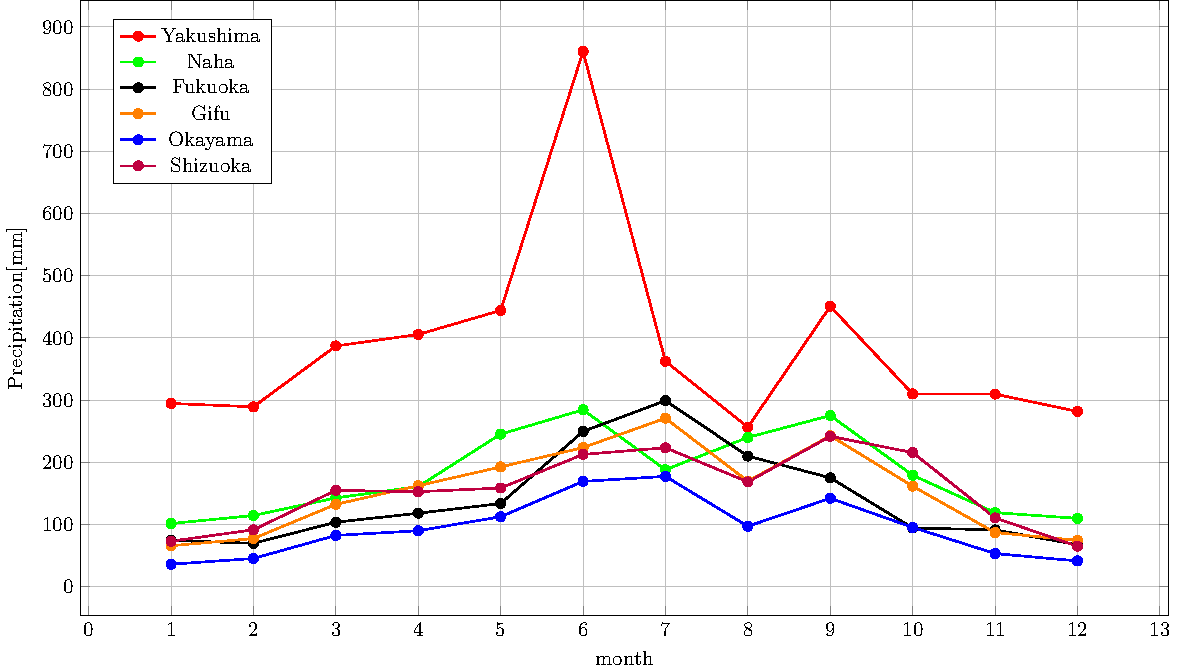
\includegraphics[width=\linewidth]{chap_graph1.pdf}
      \caption{屋久島と各地の降水量}
      \label{fig:yakushima_precipitation}
    \end{figure}
    \vspace{-2em}
    \begin{table}[H]
      \centering
      \begin{tabular}{|c|c|c|c|c|c|}
         \hline
          屋久島 & 那覇 & 福岡 & 岐阜 & 岡山 & 静岡 \\
          \hline
          4651.7 & 2161 & 1686.9 & 1860.7 & 1143.1 & 1868.2 \\\hline
      \end{tabular}
      \caption{屋久島と各地の年間降水量(単位:mm)}
      \label{tab:yakushima_precipitation}
    \end{table}
    \cref{fig:yakushima_precipitation}のグラフを見てわかる通り, 屋久島の降水量は他の地域と比べて圧倒的に多い.
    また, \cref{tab:yakushima_precipitation}を見ると, 年間降水量ではほかの地域の2倍以上の降水量があることがわかる.
    また, 山間部では2012年に屋久杉ランドで11130mm(平年値:10048mm)の降水量を記録した. これは世界最多とされるチェラプランジ(インド)の平年値である10449mmに迫る.屋久島は世界でも有数の豪雨地帯であるのだ.
  \section{屋久島の気温}
    屋久島の気温は年間を通して温暖で, 年平均気温は約19.6℃である. もっとも気温が低い一月でも平均気温は約11.8℃と気温は低くても8℃程度である.
    ただし, 山間部では標高が高くなるにつれて気温が低くなり, 山頂付近では年平均気温が6-7℃程度と北海道旭川と同程度の気温になる.
    この気温差が屋久島の大きな特徴である垂直分布\footnotemark[5] を生み出している.
    \footnotetext[5]{chapter3を参照}
\end{document}